%-----------------------------------------------------------------------------------------------------------------------------------------------%
%	The MIT License (MIT)
%
%	Copyright (c) 2015 Jan Küster
%
%	Permission is hereby granted, free of charge, to any person obtaining a copy
%	of this software and associated documentation files (the "Software"), to deal
%	in the Software without restriction, including without limitation the rights
%	to use, copy, modify, merge, publish, distribute, sublicense, and/or sell
%	copies of the Software, and to permit persons to whom the Software is
%	furnished to do so, subject to the following conditions:
%	
%	THE SOFTWARE IS PROVIDED "AS IS", WITHOUT WARRANTY OF ANY KIND, EXPRESS OR
%	IMPLIED, INCLUDING BUT NOT LIMITED TO THE WARRANTIES OF MERCHANTABILITY,
%	FITNESS FOR A PARTICULAR PURPOSE AND NONINFRINGEMENT. IN NO EVENT SHALL THE
%	AUTHORS OR COPYRIGHT HOLDERS BE LIABLE FOR ANY CLAIM, DAMAGES OR OTHER
%	LIABILITY, WHETHER IN AN ACTION OF CONTRACT, TORT OR OTHERWISE, ARISING FROM,
%	OUT OF OR IN CONNECTION WITH THE SOFTWARE OR THE USE OR OTHER DEALINGS IN
%	THE SOFTWARE.
%	
%
%-----------------------------------------------------------------------------------------------------------------------------------------------%


%============================================================================%
%
%	DOCUMENT DEFINITION
%
%============================================================================%

%we use article class because we want to fully customize the page and dont use a cv template
\documentclass[10pt,A4]{article}	


%----------------------------------------------------------------------------------------
%	ENCODING
%----------------------------------------------------------------------------------------

%we use utf8 since we want to build from any machine
\usepackage[utf8]{inputenc}		

%----------------------------------------------------------------------------------------
%	LOGIC
%----------------------------------------------------------------------------------------

% provides \isempty test
\usepackage{xifthen}

%----------------------------------------------------------------------------------------
%	FONT
%----------------------------------------------------------------------------------------

% some tex-live fonts - choose your own

%\usepackage[defaultsans]{droidsans}
%\usepackage[default]{comfortaa}
%\usepackage{cmbright}
%\usepackage[default]{raleway}
%\usepackage{fetamont}
%\usepackage[default]{gillius}
%\usepackage[light,math]{iwona}
%\usepackage[thin]{roboto} 

% set font default
\renewcommand*\familydefault{\sfdefault} 	
\usepackage[T1]{fontenc}

% more font size definitions
\usepackage{moresize}		


%----------------------------------------------------------------------------------------
%	PAGE LAYOUT  DEFINITIONS
%----------------------------------------------------------------------------------------

%debug page outer frames
%\usepackage{showframe}			


%define page styles using geometry
\usepackage[a4paper]{geometry}		

% for example, change the margins to 2 inches all round
\geometry{top=.5cm, bottom=-.6cm, left=-0.1cm, right=0cm} 	

%use customized header
\usepackage{fancyhdr}				
\pagestyle{fancy}

%less space between header and content
\setlength{\headheight}{-5pt}		


%customize entries left, center and right
\lhead{}
\chead{}
\rhead{}

\newcommand{\padding}{1cm}
\newcommand{\innerwidth}{\linewidth-\padding-\padding}

%indentation is zero
\setlength{\parindent}{0mm}

%----------------------------------------------------------------------------------------
%	TABLE /ARRAY DEFINITIONS
%---------------------------------------------------------------------------------------- 

%for layouting tables
\usepackage{multicol}			
\usepackage{multirow}

%extended aligning of tabular cells
\usepackage{array}

\newcolumntype{x}[1]{%
>{\raggedleft\hspace{0pt}}p{#1}}%


%----------------------------------------------------------------------------------------
%	GRAPHICS DEFINITIONS
%---------------------------------------------------------------------------------------- 

%for header image
\usepackage{graphicx}

%for floating figures
\usepackage{wrapfig}
\usepackage{float}
%\floatstyle{boxed} 
%\restylefloat{figure}

%for drawing graphics		
\usepackage{tikz}				
\usetikzlibrary{shapes, backgrounds,mindmap, trees}


%----------------------------------------------------------------------------------------
%	Color DEFINITIONS
%---------------------------------------------------------------------------------------- 
\usepackage{transparent}
\usepackage{color}

%accent color
\definecolor{sectcol}{RGB}{255,150,0}

%dark background color
\definecolor{bgcol}{RGB}{110,110,110}

%light background / accent color
\definecolor{softcol}{RGB}{225,225,225}

% light bg
\definecolor{light}{RGB}{210, 210, 210}

%============================================================================%
%
%
%	DEFINITIONS
%
%
%============================================================================%

%----------------------------------------------------------------------------------------
% 	HEADER
%----------------------------------------------------------------------------------------

% remove top header line
\renewcommand{\headrulewidth}{0pt} 

%remove botttom header line
\renewcommand{\footrulewidth}{0pt}	  	

%remove pagenum
\renewcommand{\thepage}{}	

%remove section num		
\renewcommand{\thesection}{}			

%----------------------------------------------------------------------------------------
% 	ARROW GRAPHICS in Tikz
%----------------------------------------------------------------------------------------

% a six pointed arrow poiting to the left
\newcommand{\tzlarrow}{(0,0) -- (0.2,0) -- (0.3,0.2) -- (0.2,0.4) -- (0,0.4) -- (0.1,0.2) -- cycle;}	

% include the left arrow into a tikz picture
% param1: fill color
%
\newcommand{\larrow}[1]
{\begin{tikzpicture}[scale=0.58]
	 \filldraw[fill=#1!100,draw=#1!100!black]  \tzlarrow
 \end{tikzpicture}
}

% a six pointed arrow poiting to the right
\newcommand{\tzrarrow}{ (0,0.2) -- (0.1,0) -- (0.3,0) -- (0.2,0.2) -- (0.3,0.4) -- (0.1,0.4) -- cycle;}

% include the right arrow into a tikz picture
% param1: fill color
%
\newcommand{\rarrow}[1]
{\begin{tikzpicture}[scale=0.7]
	 \filldraw[fill=#1!100,draw=#1!100!black]  \tzrarrow
 \end{tikzpicture}
}



%----------------------------------------------------------------------------------------
%	custom sections
%----------------------------------------------------------------------------------------

% create a coloured box with arrow and title as cv section headline
% param 1: section title
%
\newcommand{\cvsection}[1]
{
\colorbox{sectcol}{\mystrut \makebox[1\linewidth][l]{
\larrow{bgcol} \hspace{-8pt} \larrow{bgcol} \hspace{-8pt} \larrow{bgcol} \textcolor{white}{\textbf{#1}}\hspace{4pt}
}}\\
}

%create a coloured arrow with title as cv meta section section
% param 1: meta section title
%
\newcommand{\metasection}[2]
{
\begin{tabular*}{1\textwidth}{p{2cm} p{11cm}}
\larrow{bgcol}	\normalsize{\textcolor{sectcol}{#1}}&#2\\[8pt]
\end{tabular*}
}

%----------------------------------------------------------------------------------------
%	 CV EVENT
%----------------------------------------------------------------------------------------

% creates a stretched box as cv entry headline followed by two paragraphs about 
% the work you did
% param 1:	event time i.e. 2014 or 2011-2014 etc.
% param 2:	event name (what did you do?)
% param 3:	institution (where did you work / study)
% param 4:	what was your position
% param 5:	some words about your contributions
%
\newcommand{\cvevent}[5]
{
\vspace{8pt}
	\begin{tabular*}{0.6\linewidth}{ p{12cm} x{3cm}}
\textbf{#2} \textcolor{bgcol}{(#3)}&\textcolor{bgcol}{#1}\\[4pt]
	\end{tabular*}
\vspace{-12pt}
\textcolor{softcol}{\hrule}
\vspace{6pt}
	\begin{tabular*}{1\textwidth}{l}
		 \larrow{sectcol}  #4\\[4.5pt]
		 \larrow{sectcol}  #5\\[6pt]
	\end{tabular*}
\vspace{-4pt}
}

% creates a stretched box as 
\newcommand{\cveventmeta}[2]
{
	\mbox{\mystrut \hspace{87pt}\textit{#1}}\\
	#2
}

%----------------------------------------------------------------------------------------
% CUSTOM STRUT FOR EMPTY BOXES
%----------------------------------------- -----------------------------------------------
\newcommand{\mystrut}{\rule[-.3\baselineskip]{0pt}{\baselineskip}}

%----------------------------------------------------------------------------------------
% CUSTOM LOREM IPSUM
%----------------------------------------------------------------------------------------
\newcommand{\lorem}
{Lorem ipsum dolor sit amet, consectetur adipiscing elit. Donec a diam lectus.}



%============================================================================%
%
%
%
%	DOCUMENT CONTENT
%
%
%
%============================================================================%
\begin{document}

%use our custom fancy header definitions
\pagestyle{fancy}	

%----------------------------------------------------------------------------------------
% HEADLINE / BASIC INFORMATION
%----------------------------------------------------------------------------------------
\fcolorbox{bgcol}{bgcol}{
\begin{minipage}[c][0.085\textheight][t]{\linewidth}
\begin{center}
	\vspace{14pt}
	\textcolor{light}{\small{Software Engineer $\cdot$  Bengaluru, India  $\cdot$  sudharpun90@gmail.com  $\cdot$ +91 9677099477}}\\
	\HUGE{\textcolor{white}{\textsc{Sudharshan Krishnakumar}} } %\textcolor{sectcol}{\rule[-1mm]{1mm}{0.9cm}} \HUGE{\textcolor{white}{\textsc{Resume}} }
\end{center}
\end{minipage}}\\[-4pt]
%----------------------------------------------------------------------------------------
% SUMMARY
%----------------------------------------------------------------------------------------
\fcolorbox{sectcol}{sectcol}{
\begin{minipage}[c][0.03\textheight][t]{\linewidth}
\vspace{-3pt}
\begin{center}
\parbox[b]{0.75\linewidth}{
	\begin{center}
	\large
	\larrow{bgcol}\larrow{bgcol} \textcolor{white}{I like to build intelligent  components that could be re-used and scaled.} \rarrow{bgcol}\rarrow{bgcol}
	\end{center}
}
\end{center}
\end{minipage}}\\[-4pt]
%----------------------------------------------------------------------------------------
% META
%----------------------------------------------------------------------------------------
\fcolorbox{white}{white}{
\begin{minipage}[c][0.16\textheight][t]{\linewidth}
\vspace{8pt}
\begin{center}
\parbox[c]{\innerwidth}{
	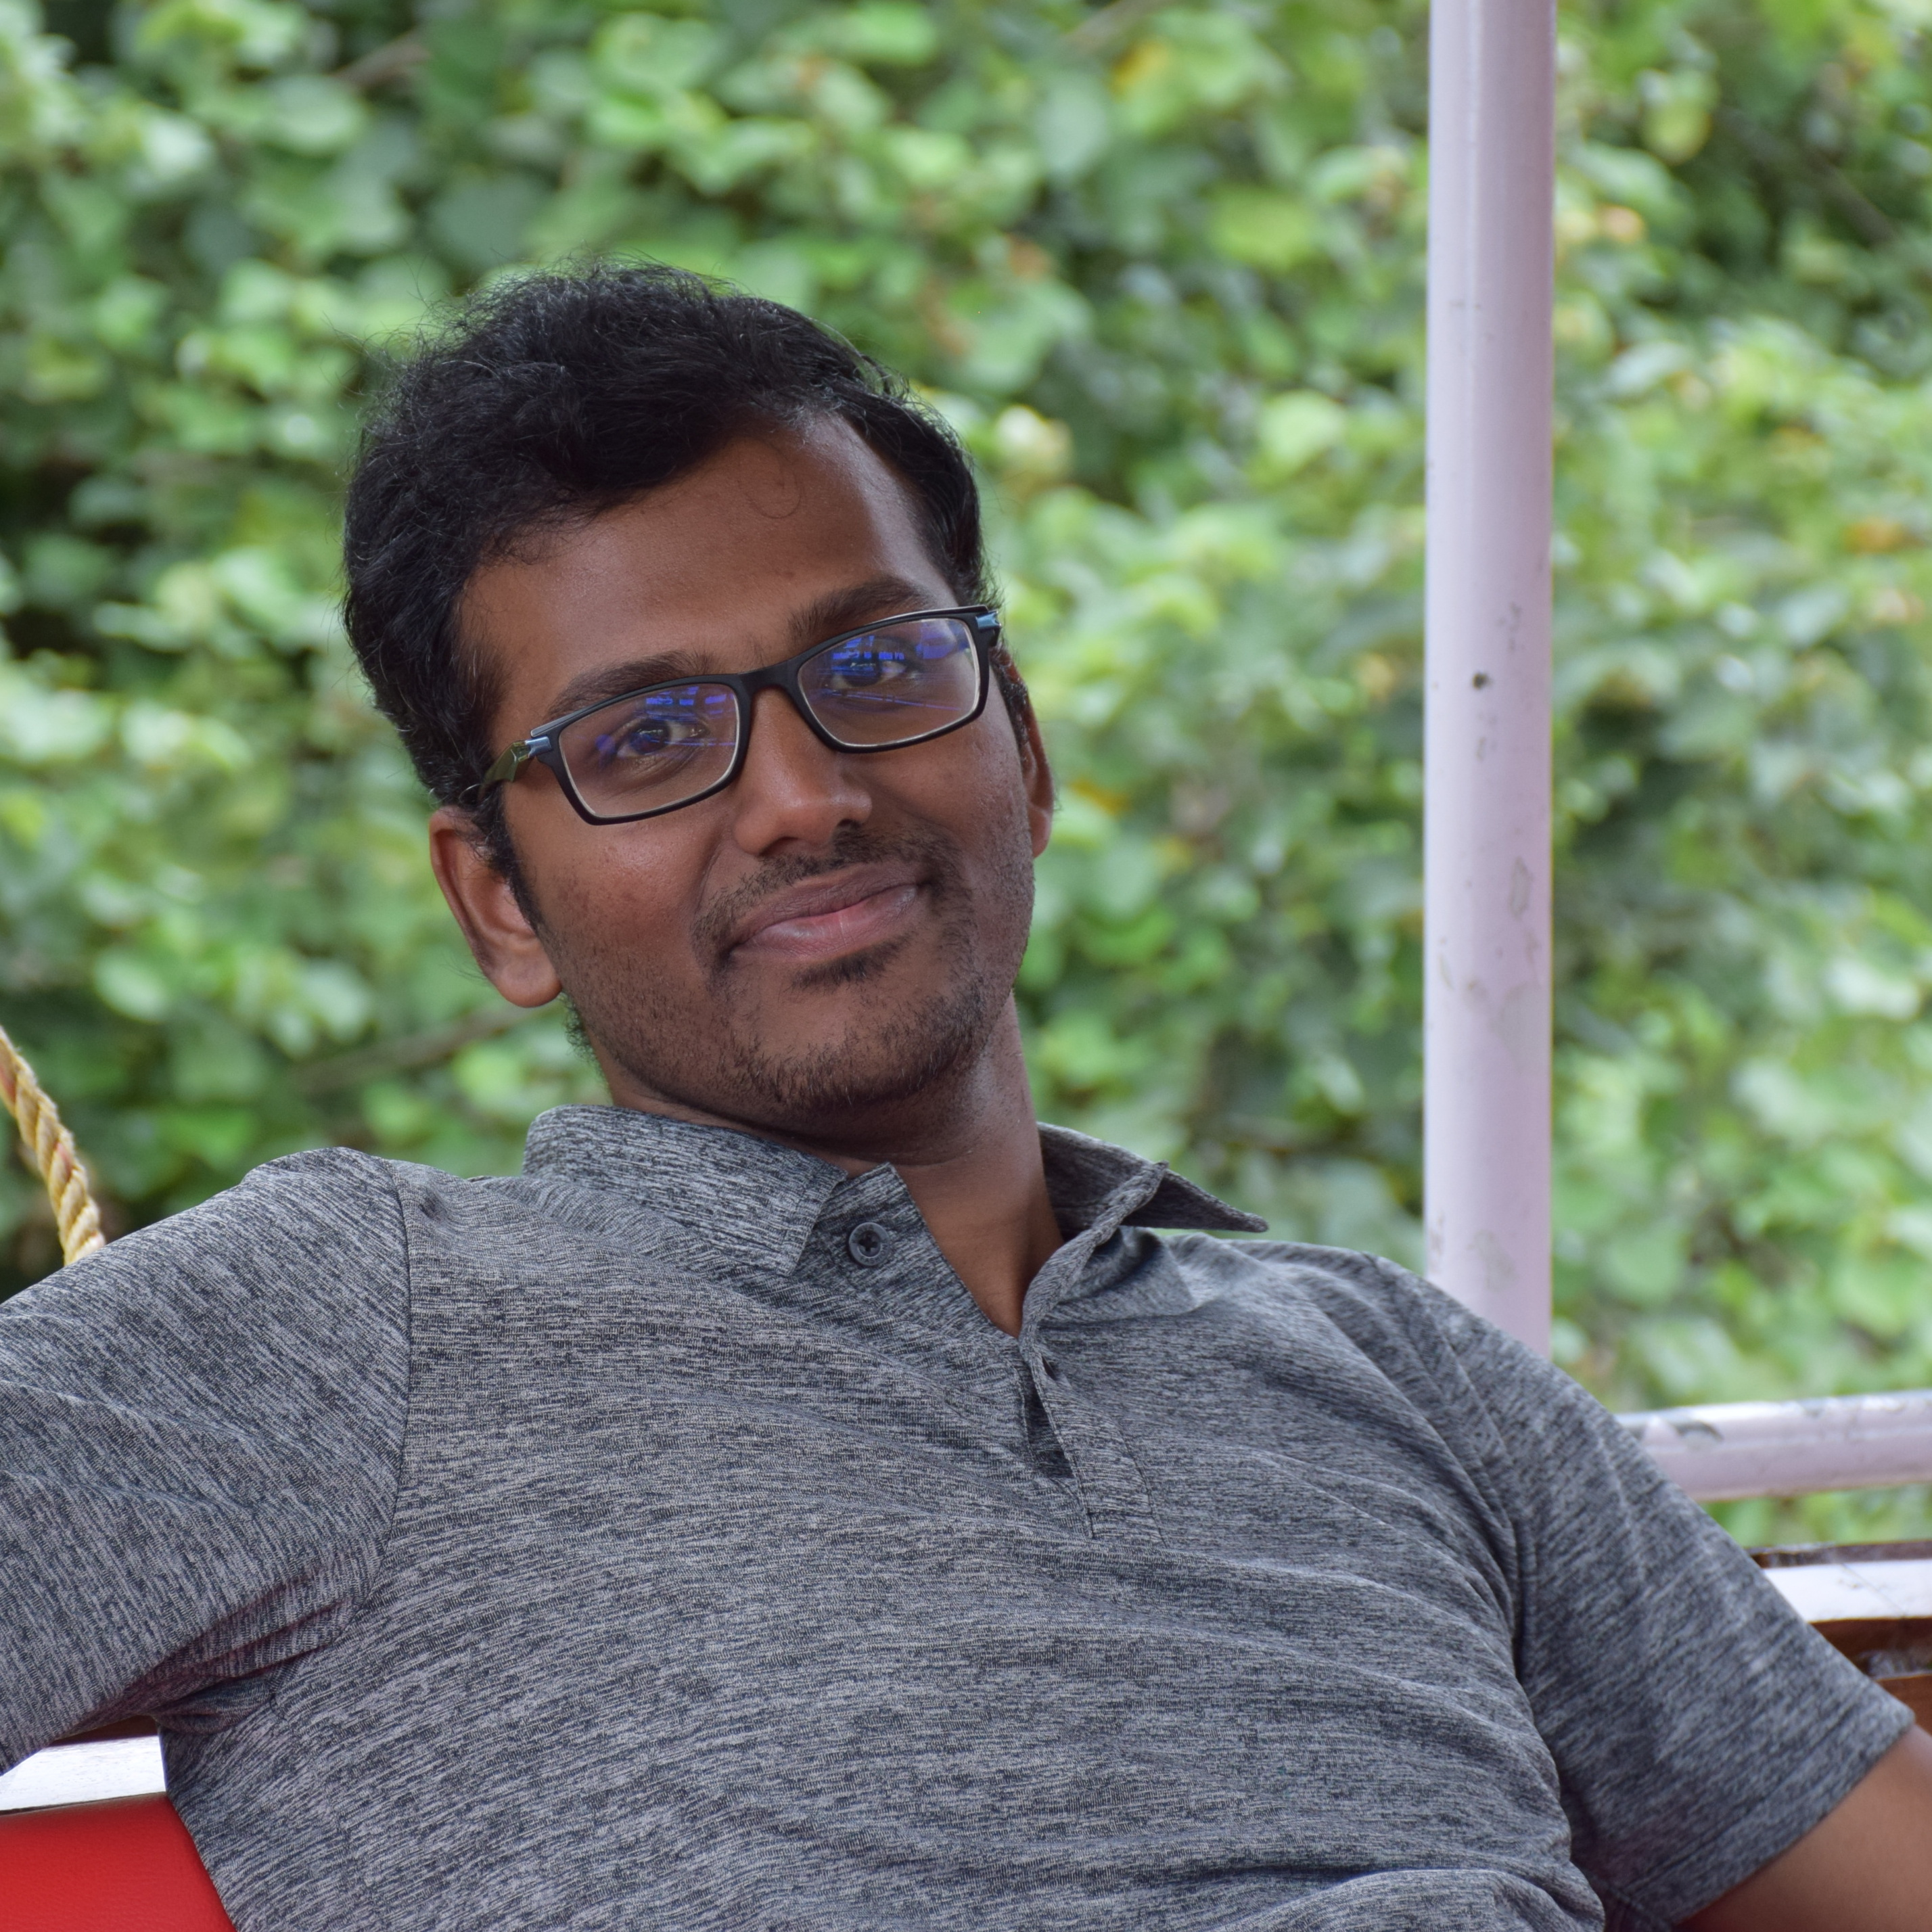
\includegraphics[width=120pt,height=120pt,keepaspectratio]{myfoto.jpg}
	\hspace{8pt}
	\parbox[b]{5cm}{
	\metasection{Status:}{Staff Big Data Engineer, Masters in Computer Science}
	\metasection{Stack:}{Kafka, Spark, Spark Streaming, Spark on Kubernetes,   }
		\metasection{Languages:}{Java, Scala, Python, Shell Scripting, R}
	\metasection{Tools:}{IntelliJ, PyCharm, Git, Ansible, Jenkins}
	}
}
\end{center}
\end{minipage}}\\[-4pt]
%----------------------------------------------------------------------------------------
% EXPERIENCE
%----------------------------------------------------------------------------------------
\fcolorbox{light}{light}{
\begin{minipage}[c][0.36\textheight][t]{\linewidth}
\vspace{4pt}
\hspace{26pt}
\parbox[c]{0.75\linewidth}{
%
\cvevent{2020 - now}{Staff Software Engineer}{Visa - Realtime Processing}{Refactoring of realtime processing code by segmenting it based on functionality.}{Built code for pluggable transformations, to support continuous execution of realtime pipeline.}

\textcolor{softcol}{\hrule}

\cvevent{2018 - 2019}{Staff Software Engineer}{Visa - Data Localization}{Enabling single click deployment with regional configuration support.}{Enabling pipeline for Spark on kubernetes for compute intensive tasks.}


\textcolor{softcol}{\hrule}

\cvevent{2015 - 2018}{Senior Software Engineer}{Visa - Hadoop Transformation}{Developed generic frameworks to enable transformation towards Hadoop and spark ecosystem}{Built migration tools like Dataset comparator,  Reference Analyzer for speedy migration}
\textcolor{softcol}{\hrule}


\cvevent{2012 - 2013}{Senior Software Engineer}{Persistent System - Connector Development} {Developed connectors for different platform (CRM, ERP and Social platforms)}{Built generic parsing module to parse responses (XML,JSON,CSV) and generate relational data}

%\textcolor{softcol}{\hrule}


%\cvevent{2011 - 2012}{Software Engineer}{Persistent System - Ticket breach prediction}{Built UI tool to present SLA breach prediction of service ticket to the call center dispatchers.}{Developed code in java for testing data from PMML to remove the dependency on expensive toolkit.}

\textcolor{softcol}{\hrule}
}
\hspace{18pt}
\textcolor{sectcol}{\rule[-3.2cm]{2pt}{7cm}}
\hspace{12pt}
\rotatebox[origin=c]{270}{\HUGE \textsc{Experience}}
\end{minipage}}\\[-4pt]


%----------------------------------------------------------------------------------------
% Github
%----------------------------------------------------------------------------------------
\fcolorbox{bgcol}{bgcol}{
\begin{minipage}[c][0.03\textheight][t]{\linewidth}
\vspace{-3pt}
\begin{center}
\parbox[b]{0.75\linewidth}{
	\begin{center}
	\large
	\textcolor{white}{Check out my projects at - } \textcolor{sectcol}{\textbf{github.com/sudhargk}}
	\end{center}
}
\end{center}
\end{minipage}}\\[-4pt]
%----------------------------------------------------------------------------------------
% Projects
%----------------------------------------------------------------------------------------
\fcolorbox{white}{white}{
\begin{minipage}[c][0.2875\textheight][t]{\linewidth}
\vspace{1pt}
\hspace{26pt}
\parbox[c]{0.75\linewidth}{

\cvevent{2018 - 2019}{NSDC Insight - R-Shiny Dashboard}{Univerity of Chicago}{Built a R Shiny UI app for preprocessing, visualizaiion and prediction on NSDC dataset.}{User friendly control to upload dataset, pre-process and predict.}

%\textcolor{softcol}{\hrule}

\cvevent{2014 - 2015}{Automatic video annotation - sudhargk/video-annotator}{IIT Madras}{Designing algorithms for extracting the semantic events in the video using deep learning.}{Generating the annotation by studying
the co-occurrence of events and objects in a given time frame.}

%\textcolor{softcol}{\hrule}


%\textcolor{softcol}{\hrule}

\cvevent{2014}{Deep Neural Net Toolbox - iitm-donlab/python-dnn}{IIT Madras}{Built a python tool-kit for deep learning algorithms using the python theano library.}{Provides easy configuration for new dataset, supports most of the variations in deep learning literature.}

%\textcolor{softcol}{\hrule}
\cvevent{2014}{Spotting of optimal business location - sudhargk/datamining}{IIT Madras}{Designed a machine learning solution to identify the desired location using social networking data.}{Implemented multiple regression techniques and achieved 81 percent accuracy on cross-validation.}

}
\hspace{18pt}
\textcolor{sectcol}{\rule[-3.2cm]{2pt}{7cm}}
\hspace{12pt}
\rotatebox[origin=c]{270}{\HUGE \textsc{Projects}}
\end{minipage}}\\[-4pt]



%----------------------------------------------------------------------------------------
% Certification
%----------------------------------------------------------------------------------------
\fcolorbox{light}{light}{
\begin{minipage}[c][0.2875\textheight][t]{\linewidth}
\vspace{1pt}
\hspace{26pt}
\parbox[c]{0.75\linewidth}{

\cvevent{2020 - Now}{Advanced Certification for Cloud, Blockchain and IoT}{IIT Madras}{Implemented course project using MQTT, AWS component viz. Dynamo DB, Kinesis, SNS.}{Advance concepts on distributed system processing viz. Consensus protocol, CAP theorem}

%\textcolor{softcol}{\hrule}

\cvevent{2018 - 2019}{Post Graduate in Data Science and Machine Learning}{Univerity of Chicago}{Learnt Data Understanding and Preparation, Analytics with R, Adavacnce Analytics and Machine Learning.}{Built a R Shiny UI app for preprocessing, visualizaiion and prediction on NSDC dataset.}

}
\hspace{18pt}
\textcolor{sectcol}{\rule[-3.2cm]{2pt}{7cm}}
\hspace{12pt}
\rotatebox[origin=c]{270}{\HUGE \textsc{Certification}}
\end{minipage}}\\[-4pt]

%----------------------------------------------------------------------------------------
% Other Interests
%----------------------------------------------------------------------------------------
\fcolorbox{sectcol}{sectcol}{
\begin{minipage}[c][0.03\textheight][t]{\linewidth}
\vspace{-3pt}
\begin{center}
\parbox[b]{0.75\linewidth}{
	\begin{center}
	\large
	\textcolor{white}{Other interests - listen to classical music \& reading biographiesa and research papers.}
	\end{center}
}
\end{center}
\end{minipage}}\\[-4pt]

%----------------------------------------------------------------------------------------
% Education
%----------------------------------------------------------------------------------------
\fcolorbox{white}{white}{
\begin{minipage}[c][0.2875\textheight][t]{\linewidth}
\vspace{1pt}
\hspace{12pt}
%\parbox[c]{0.75\linewidth}{
%\cvevent{2015}{Master of Technology,Indian Institute of Technology, Madras}{CGPA : 9.6}
%\cvevent{2011}{Bachelor of Engineering, MES College of Engineering, Pune}{Percent : 75.8}
%}
\begin{tabular}{||c c c c||} 
 \hline
 \large	
  \textbf{Program} &  \textbf{Institution} &  \textbf{CGPA/Percent} &  \textbf{Year of Completion} \\ [1ex] 
 \hline\hline
 Master of Technology & Indian Institute of Technology, Madras & 9.6 & 2015 \\ 
 Bachelor of Engineering & MES College of Engineering, Pune & 75.8\% & 2011 \\
 XII\textsuperscript{th} Std. (CBSE) & Kendriya Vidyalaya Ganeshkhind, Pune & 90.2\% & 2007 \\ 26pt
 X\textsuperscript{th} Std. (CBSE) & Kendriya Vidyalaya Ganeshkhind, Pune & 83.8\% & 2005 \\
\hline
\end{tabular}
\hspace{18pt}
\textcolor{sectcol}{\rule[-3.2cm]{2pt}{7cm}}
\hspace{12pt}
\rotatebox[origin=c]{270}{\HUGE \textsc{Education}}
\end{minipage}}\\[-4pt]

%-------------------------------------------------------------------------------------------------
% FOOTER
%--------------------------------------------------------------------------------------------------
\fcolorbox{bgcol}{bgcol}{
\begin{minipage}[c][0.01\textheight][t]{\linewidth}
\vspace{-8pt}
\begin{center}
\parbox[b]{0.75\linewidth}{
\begin{center}\textcolor{white}{`Learning never exhausts the mind` - Leonardo da Vinci}\end{center}
}
\end{center}
\end{minipage}}
%============================================================================%
%
%
%
%	DOCUMENT END
%
%
%
%============================================================================%
\end{document}
